\chapter{Autonomous flight}
The following sections introduces the selection, set up and how autonomous flight was achieved.

\section{Drone selection}
To fulfil the vision of and easy to use and readily available drone platforms the drone selection could be narrowed down quite easily. As the primary focus of the of the project was to explore autonomous flight other concerns such as resistance to rough weather could be neglected. \\
During the course 2 drones matching the giving requirements were introduced: The dji Phantom 2 \cite{Ref:dji} and the 3DR Iris+ \cite{Ref:3dr}.\\
The obvious choice between the 2 drones was the Iris+ as it used the open source Pixhawk FCU \cite{Ref:px4}. Having an open source FCU allowed for easy interfacing and more flexibility with many tasks concerning the drone. The Iris+ drone can be seen on figure \ref{fig:iris}.\\

The main features and components of the Iris+ drone used for this project are:
\begin{itemize}
\item 16-22 minutes flight time.
\item Payload capacity of 400g.
\item Manual remote control.
\item Telemetry link.
\item Autonomous way point navigation.
\item Feature rich ground control software.
\end{itemize}

\begin{figure}[H]
  \centering
    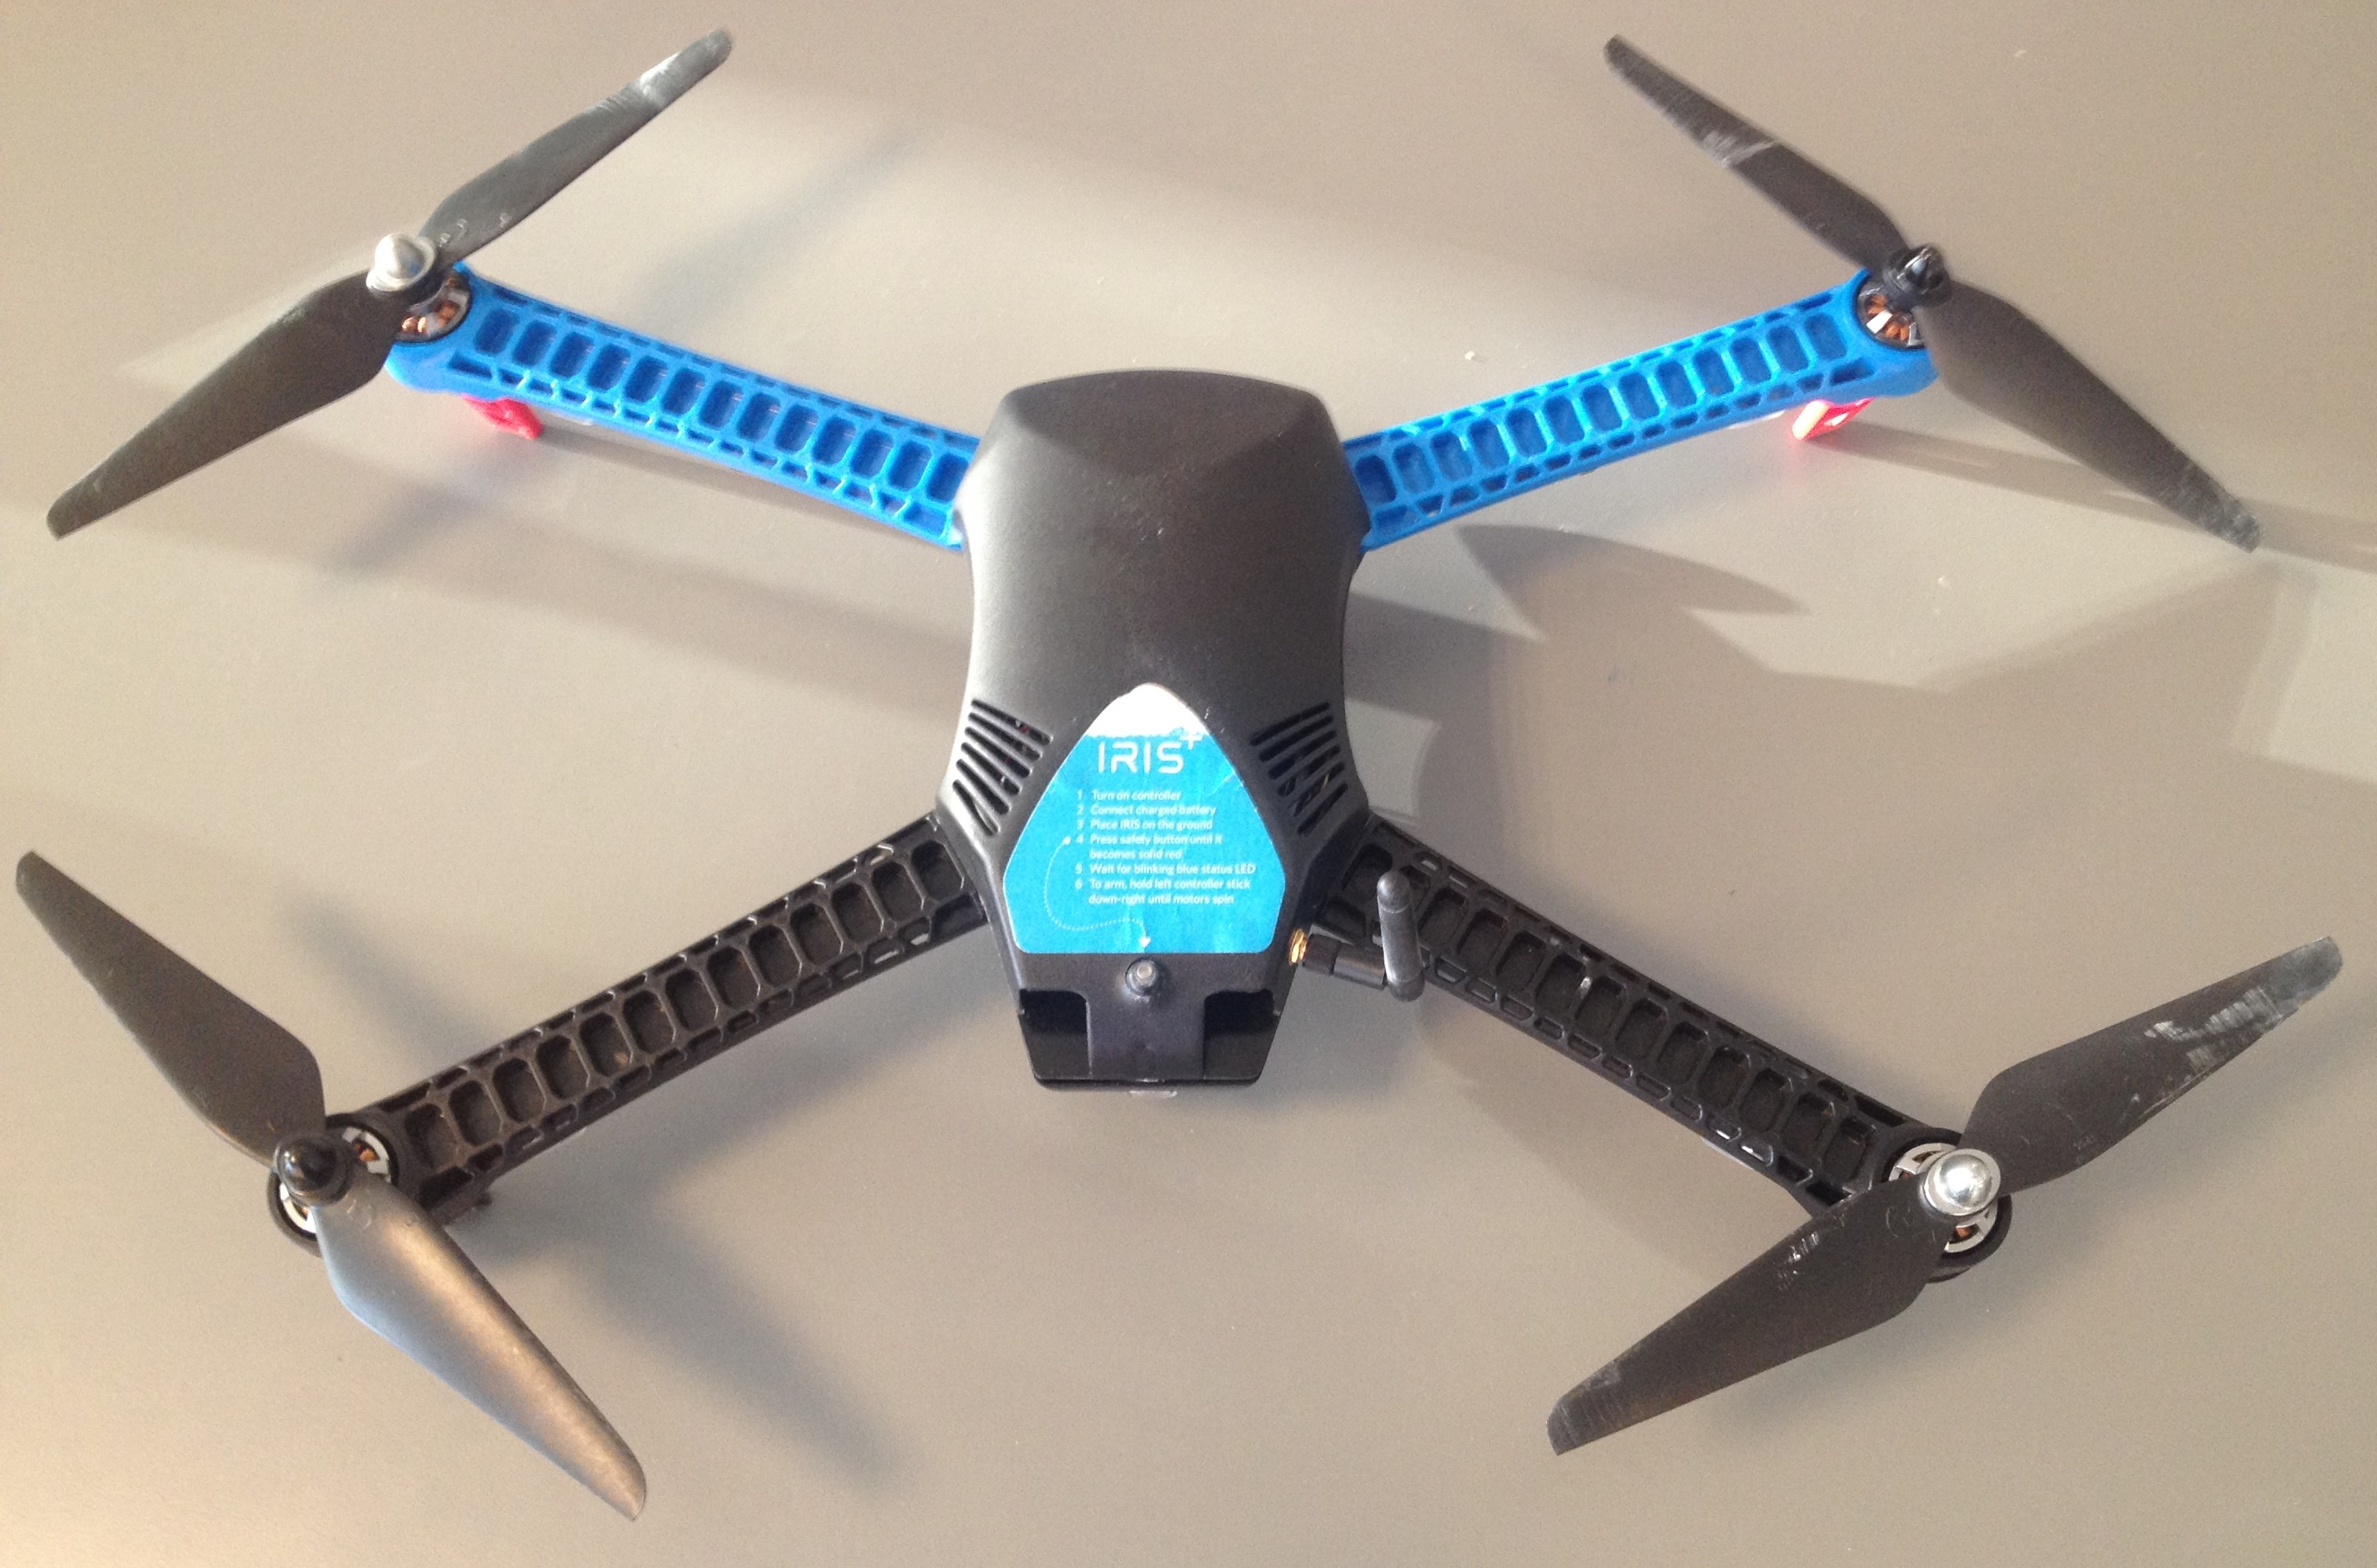
\includegraphics[width=0.65\textwidth]{./Images/iris}
  \caption{TThe Iris+ drone.}
  \label{fig:iris}
\end{figure}


\section{Setup}
\subsection*{Radio Controller}
The first part of the set up was to bind the Radio Controller. The receiver used is the $2.4 Ghz$ Frsky D4R-2 Reciever \cite{Ref:FrSky} and can be seen on figure \ref{fig:irisInside}\\ 
To bind the controller the hood of the drone had to be taken off to access the radio receiver. Then the steps are as follows:
\begin{itemize}
\item[1.] Turn on the radio transmitter while down the button on the back of the radio transmitter.
\item[2.] Once the remote is beeping let go of the button on the back.
\item[3.] Power up the drone while holding down the F/S button on the radio receiver.
\item[4.] Release the F/S button once the radio receiver LED is flashing red and green.
\item[5.] Power off drone.
\item[6.] Power off radio transmitter.
\item[7.] If bind is done correctly the radio receiver LED should be solid green when connected to the radio transmitter and the LED blink red when data is transferred.
\end{itemize}
For further assistance the first part of the following video i suggested \url{https://www.youtube.com/watch?v=5ygCbdR4FCE}.

\begin{figure}[H]
  \centering
    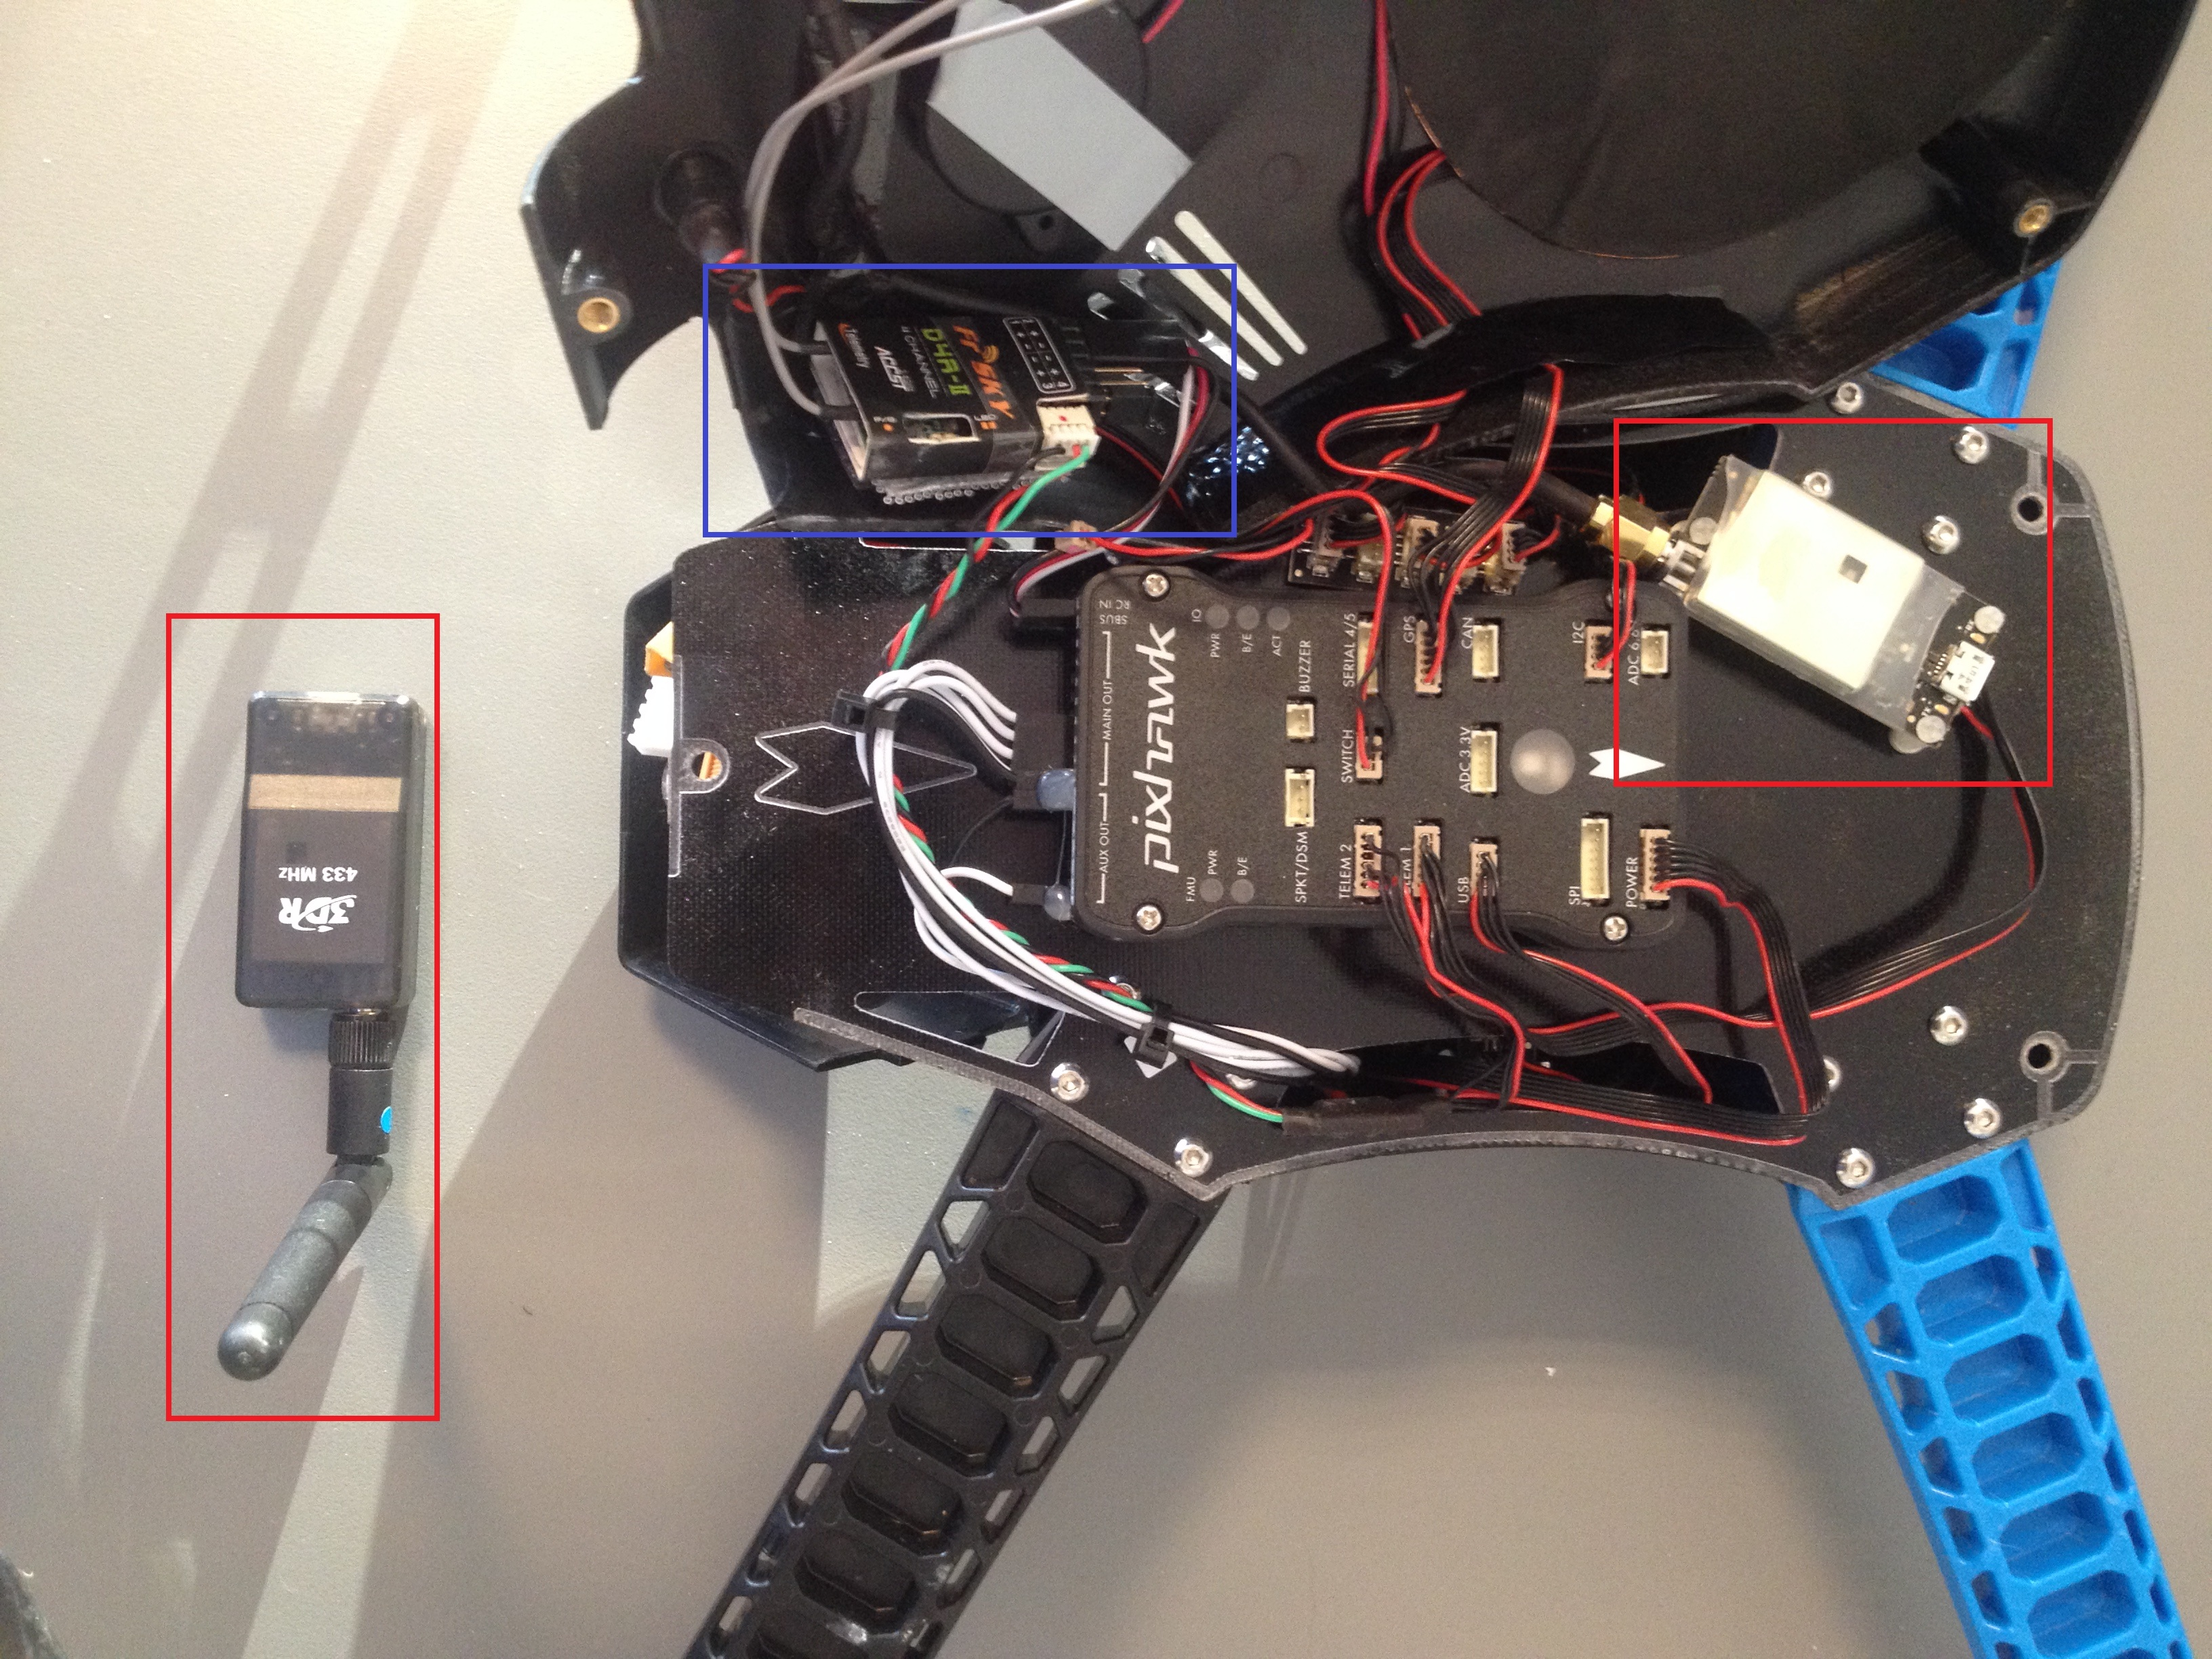
\includegraphics[width=0.65\textwidth]{./Images/insideIRIS}
  \caption{The Iris+ drone inside.The red rectangles marks the telemetry and the blue rectangle mark the radio receiver.}
  \label{fig:irisInside}
\end{figure}

\subsection*{Telemetry}
The telemetry used is the 3DR Radio v2 \cite{Ref:Telem} operating at $433 Mhz$. The purpose of the telemetry is to transmit and receive data from and to the ground station via the MAVLink protocol \cite{Ref:MAVLink}.\\
To connect the ground telemetry to the telemetry on the drone the 3DRRadio software was used on a windows machine. The two telemetries were connected to the PC by USB one at a time and set to the desired configuration. The configuration used can be seen on figure \ref{fig:telem}, where the most significant are the baud rate and the net id. When setting the configurations on the drone telemetry it is important that it is not connected to the pixhawk FCU.\\
When connected the green LED should be solid and the red LED should blink whenever data is transferred. The drone telemetry can now safely be connected to the pixhawk FCU again.

\begin{figure}[H]
  \centering
    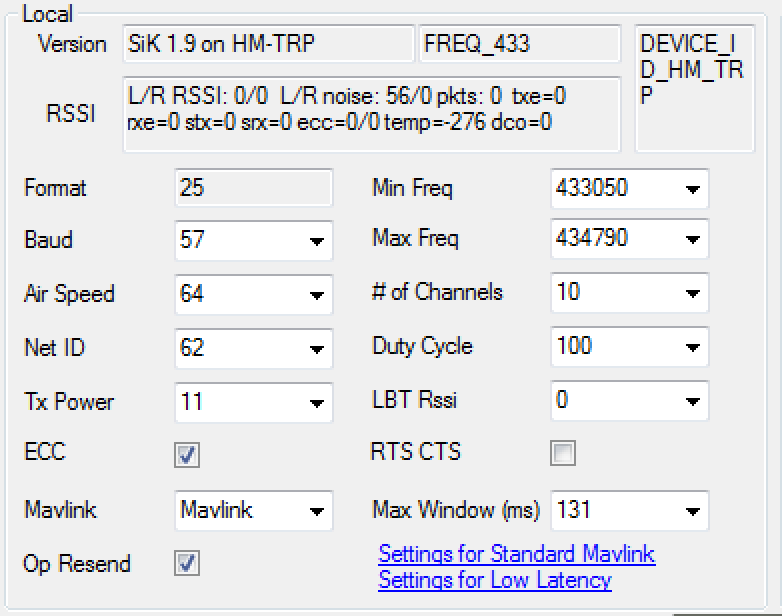
\includegraphics[width=0.65\textwidth]{./Images/telem}
  \caption{Used telemetry configurations.}
  \label{fig:telem}
\end{figure}

\subsection*{Gimbal}
Since pictures had to be taken during flight and as these pictures had to be good enough to use computer vision on it was decided to use the Tarot T-2D Brushless Gimbal Kit \cite{Ref:Gimbal}. The gimbal adds extra weight to the drone and uses extra power from the battery to power the motors. Both of these factors leads to a significant decrease in flight time.\\
The integration and usage of the gimbal will be further explained in the vision chapter. 
\subsection*{APM Planner 2.0}
The firmware for the pixhawk was a choice between the original px4 and arducopter \cite{Ref:Arducopter}. As 3DR adviced to flash the arducopter firmware and it features several features not available through the px4, arducopter was the clear choice.\\
To communicate with the arducopter firmware for calibration purposes and as a general interface APM Planner 2.0 was used \cite{Ref:APM2}. This software was run on OSX Yosemite and proved to have several crashes during calibration and firmware flashing. The best solution found for this problem was a simple reboot. While running the flight data mode where it communicated with the drone by telemetry it was very stable and responsive.\\
The APM planner 2.0 software was primarily used for calibration and waypoint planning which was a build in feature in the arducopter firmware.\\
All of the setup for the pixhawk FCU was done under initial setup in the APM planner 2.0.

\subsection*{Calibration}

After flashing the drone with new firmware and before every flight with the drone at a new location the drone was recalibrated. A proper calibration was a key element in securing accurate and safe flight with the drone. It is of great importance that the rotors are removed doing calibrations as unpredictable behaviour sometimes can occur.\\
The 4 mandatory calibrations that had to be done were:
\begin{itemize}
\item Frame type
\item Compass calibration
\item Accelerometer calibration
\item Radio calibration
\end{itemize}

To calibrate for the physical appearance of the drone the proper frame type has to be selected. This is done under the "initial setup" menu where "Frame type" should be selected. The proper frame type is selected and then downloaded. This sets all the parameters for the specific drone type. For this project the iris+ with tarot gimbal was used.\\

The compass calibration involves rotating the drone around all axes to fill in the calibration matrix. The matrix and all the calculations are handled by APM Planner 2.0. First the pixhawk is selected in the menu and the live calibration is chosen. This will give you a minute to rotate the drone around all axes. It is advised to power the drone with battery as the wire might get tangled up and make the calibration more complicated. Sometimes several crashes were encountered doing the calibration process for no apparent reason.\\

The calibration of the accelerometer was pretty straight forward. To calibrate the the accelerometer the software asks you to put the drone in 6 distinct positions and then press enter.\\

The last mandatory calibration needed is the radio calibration. When the radio is turned on and properly connected to the drone the radio calibration can be initiated. All of the control sticks and switches are moved to its outer positions.  The process can be followed on the GUI to see if everything is working properly. After moving everything to its outer position the throttle stick is moved down while the other stick is in its center position.\\

All of these calibrations are of great importance in order to fly the iris drone properly. Several problems were encountered due to bad calibration and not checking everything without rotors. If anything seems off during the initial flight or testing without rotors it is suggested to either do a complete recalibration or re-flashing with the newest software. A guide for the mandatory calibration can be found at \url{http://copter.ardupilot.com/wiki/initial-setup/configuring-hardware/} it should however be noted that some elements are a bit outdated in this guide.

\subsection*{Flight modes}
As the arducopter firmware has several different flight modes and the pre set flight modes does not match the desired flight modes for this project they have to be changed. The desired flight modes are stabilize and auto-hold for manual modes and auto mode for autonomous flight. It is important to set these flight modes to overrule the autonomous flight if anything is not going according to plan.\\
As different radio controllers are available one should always check that the flight modes are mapped to the used controller as desired, without rotors.\\
To additional fly modes were used to easily land the drone and to return the drone to the position it was armed at. These modes were land and return to land (RTL). The land flight mode performs a landing at the current spot, disabling the throttle switch but enabling control of the position stick.\\

\subsection*{Fail safe}
To control the behaviour in case of a malfunction on the radio controller side or the drone running low on battery, the fail safe options have to be set. The software will give a warning to dismount the rotors doing this setup. This is important as the motors are controllable in this mode.\\
To do this the the throttle fail safe value is set approximately 30 below the lowest value of your throttle stick. This ensures that if radio connection is lost it will do the desired action. For our case we chose return to land.\\
The other fail safe option is when the drone battery level goes below a certain voltage it should perform the desired action. Return to land was also chosen for as this action.\\
The fail safe menu also provides sliders representing the values coming from the radio controller and the motor output. This feature was used to check if the flight modes gave the expected output to the motors.

\section{Flight}
To do a proper flight with the drone all of the pre arm actions have to be done. This involves keeping the drone in a steady position and having a good GPS lock. The drone is armed by first holding down the front red button on the drone, it is now ready to be armed, but not armed. The arming is different from controller to controller but the arming sequence on the used controller was to keep the throttle in the bottom right corner. To disarm it the throttle had to be in the bottom left corner. The pre arm errors can be looked up on the following page \url{http://copter.ardupilot.com/wiki/flying-arducopter/prearm_safety_check/}. It should be noted that arming the drone inside can be a tedious task as a good GPS lock is required.\\ 

\subsection{Preflight \& safety}
During the extended testing phase several safety procedures were established. This led to a preflight test check list.\\
The preflight checks in lab consisted off:
\begin{itemize}
\item[1.] Check firmware is the most recent stable version.
\item[2.] Do calibrations.
\item[3.] Set desired flight modes and fail safe settings.
\item[4.] Check output in different flight modes with motors on (no rotors).
\item[5.] Ensure proper connection to APM so data can be tracked in APM Planner 2.0.
\item[6.] Mount rotors and do test flight in drone cage.
\end{itemize}

The preflight checks at the airport consisted off:
\begin{itemize}
\item[1.] Do calibrations.
\item[2.] Ensure proper connection to APM so data can be tracked in APM Planner 2.0.
\item[3.] Contact tower to get clearance to fly and get wind speed.
\item[4.] Alert bystanders of flight.
\item[5.] Find spot for controlled crash i case of emergency.
\end{itemize}

\subsection{Autonomous flight}
To test out the autonomous flight feature on the arducopter frimware, APM planner 2.0 was used to plot a simple route at the airport. A route in APM Planner 2.0 was generated using way points. These way points were placed at a relative altitude to the drones home position which is the arming position. The drone would fly a straight path to the way point and wait there for a designated time. It is possible to control orientation of the drones as well as proximity to the way point before it is accepted.\\
The APM Planner 2.0 software offers a collection of other actions such as loiter, set region of interest etc. These were not used\\

 
\subsection{Tests}
The path shown on \ref{fig:HCAPath} was the one flown to test the autonomous flight. All of the way points were 8 meters above ground. The accepted distance to the way point was set to a 2 meter radius and the orientation of the drone was always in the direction of flight. 

\begin{figure}[H]
  \centering
    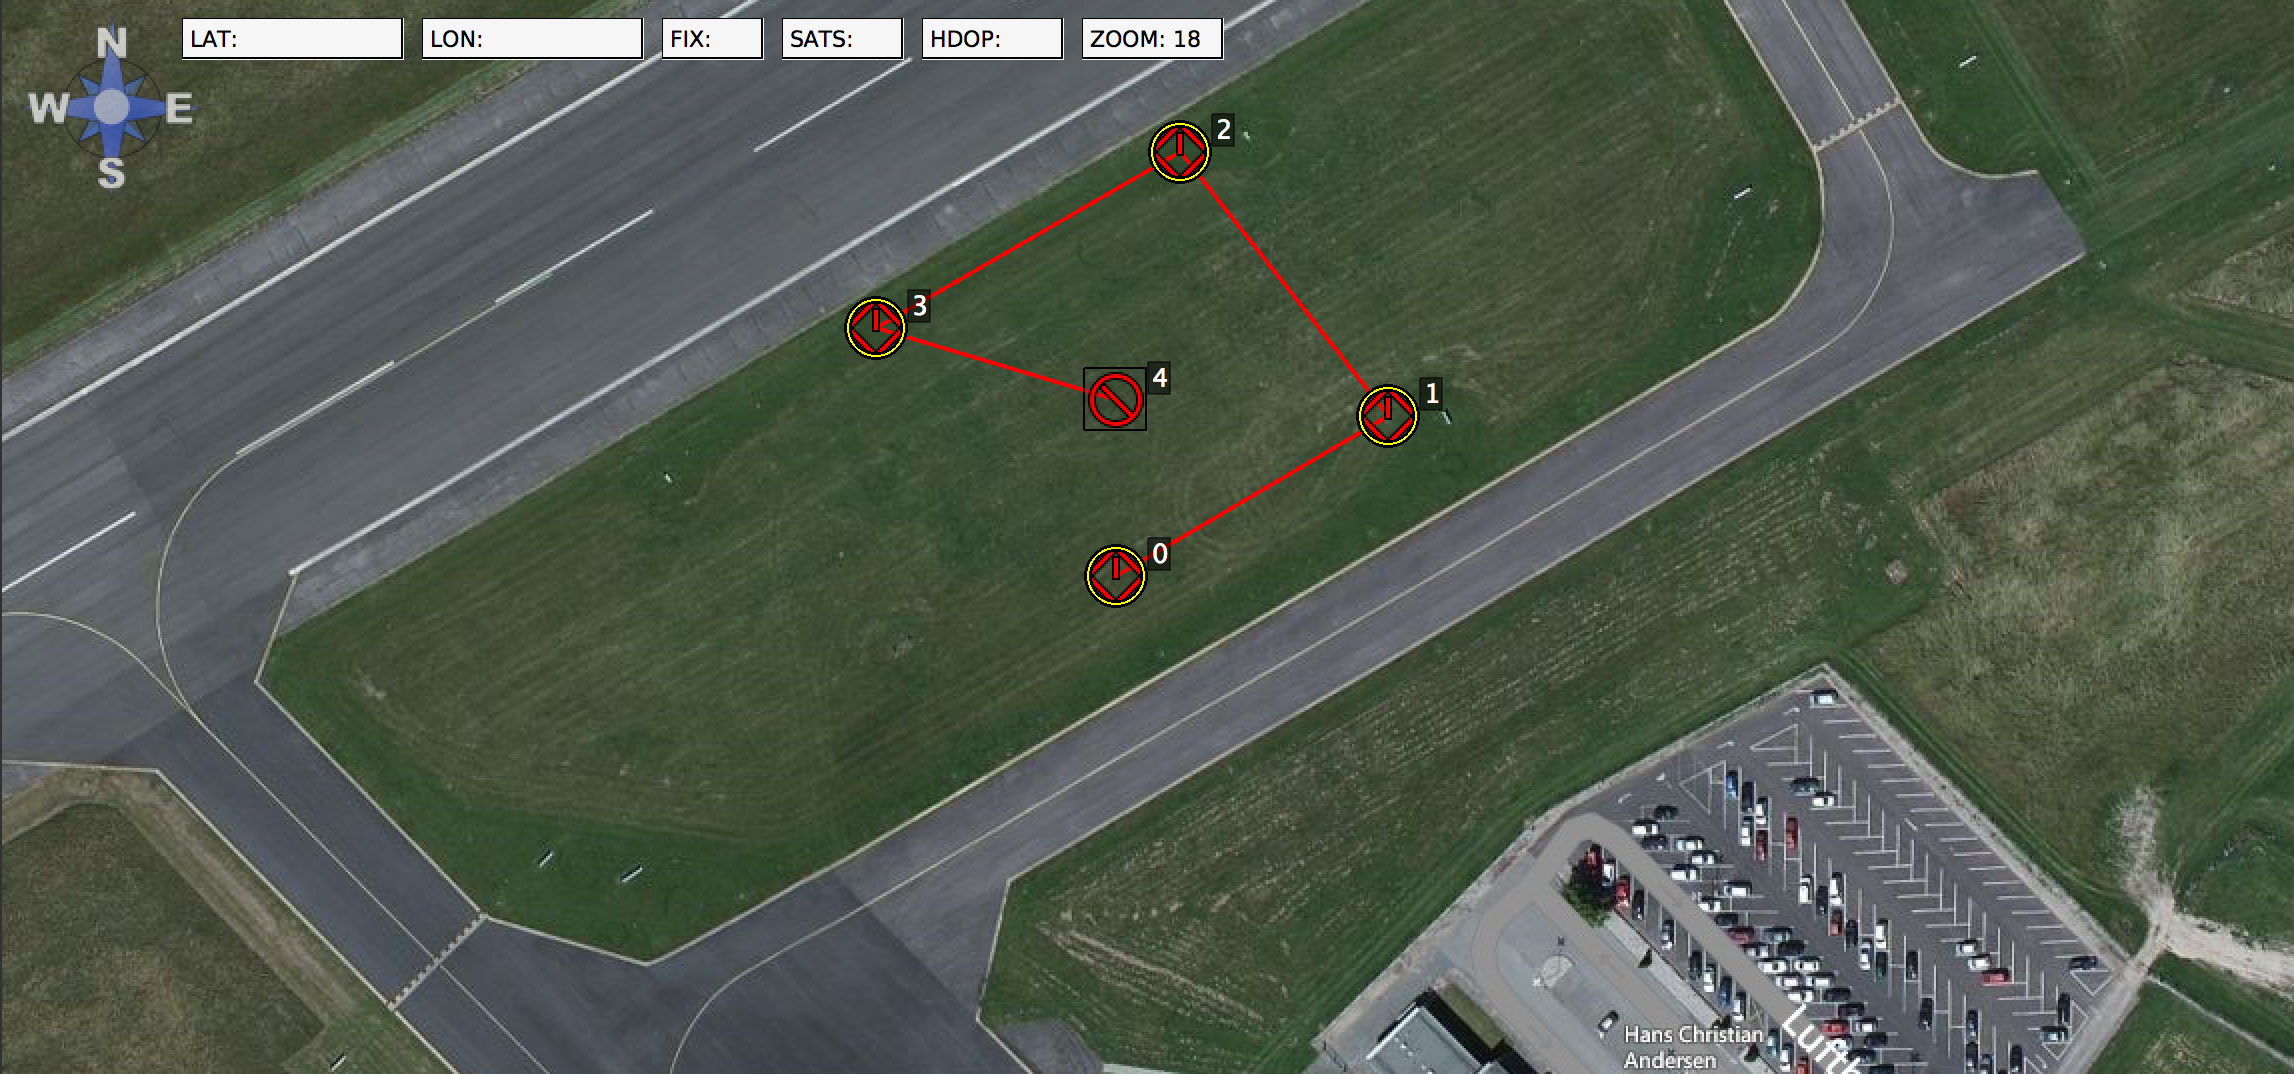
\includegraphics[width=0.95\textwidth]{./Images/HCAPath}
  \caption{Test path at HCA Airport.}
  \label{fig:HCAPath}
\end{figure}

During the test day the wind was decent which resulted in a slower flight against the wind but the overall performance of the drone was good as it flew the described route. \\

Several initial tests had been done without success due to either safety issues concerning being able to switch to manual mode and general flight planning issues.\\

One test with a altitude of 30 meters above ground was tested but had to be switched to manual mode and landed as there was too much wind.\\
 
\section{Mavros}
Since the aim of teh project was to explore autonomous flight with an easy to use interface a way to communicate directly to the drone without APM PLanner 2.0 was needed. To do this the Mavros \cite{Ref:Mavros} ros package was used. By running a main Mavros node it was possible to connect to the drones telemetry and control it.\\
As this node was in a beta state when used there was not a lot of documentation but by some trial and error it was possible to connect to the drone, arm it and upload a way point list to the pixhawk FCU. Data from the drone was also published on several topics which could be used for further control. ROS was only used on ubuntu 14.04.\\
The approach was as follow:

\begin{itemize}

\item[1.] Modify the apm2.launch files url to reflect the telemetry port and baud rate  e.g. arg name="fcu\_url" default="/dev/ttyUSB0:57600" 
\item[2.] roslaunch the modified node and verify it is connected
\item[3.] If it failed to get permission try "sudo chmod 666 /dev/ttyUSB0"
\item[4.] To enable topics streamrate from pixhawk call "rosservice call /mavros/set\_stream\_rate 0 10 1"
\item[5.] To arm use "rosservice call /mavros/cmd/arming "value: true" "
\item[6.] To load way point list use "rosrun mavros mavwp load /path/waypoints.txt" where waypoint.txt contains correct mavlink formatting.

\end{itemize}

The tests mentioned in previous section was with way points uploaded via mavros.\\
Getting the basics of uploading way points and arming the drone to work with implemented rosrun functions was simple once the syntax was mastered. Implementing this into a joint program with a path generation algorithm would be trivial. This could result in an easy to use GUI application which took a simple coordinate as an input and an altitude and the autonomously flew the drone to search.\\
The next section will describe how such a search pattern generator was developed and used.

\section{Generating search patterns}
- Mikael\\
\newpage